\documentclass[12pt]{article}

%==================== Preamble Begins ====================

%\begin{fonts}
\usepackage{mathpazo}
\usepackage{microtype}
\usepackage[utf8]{inputenc}
\usepackage{paralist}
%\end{fonts}

%\begin{layout}
\usepackage[letterpaper,margin=1in]{geometry}
\usepackage{setspace}
\onehalfspacing % Default line space is set to 1.5
\setlength{\parindent}{0pt}

\usepackage{fancyhdr} % for making fancy header/footer
\usepackage{lastpage} % for page numbering style
\pagestyle{fancy}
\fancyhf{} % clear default texts in header aned footer
\renewcommand{\headrulewidth}{0pt} % remove border line in headerb
\cfoot{Page \thepage\ of \pageref*{LastPage}} % text in center footer
%\end{layout}

%\begin{math}
\usepackage{mathtools,amsthm}
\usepackage{amssymb,nicefrac}
\usepackage{xparse} % to define \given
\DeclareMathOperator*{\argmax}{argmax}
\DeclarePairedDelimiter{\set}{\lbrace}{\rbrace} 
\DeclarePairedDelimiter{\paren}{(}{)}
\DeclarePairedDelimiter{\braket}{\langle}{\rangle}
\DeclarePairedDelimiter{\sqbrac}{[}{]}
\DeclarePairedDelimiter{\abs}{\lvert}{\rvert}
\DeclarePairedDelimiter{\norm}{\lVert}{\rVert}
\DeclarePairedDelimiter{\floor}{\lfloor}{\rfloor}
\DeclarePairedDelimiter{\ceil}{\lceil}{\rceil}
\NewDocumentCommand\given{s}{%
  \IfBooleanTF#1%
  {\;\middle\vert\;}% star version
  {\mid}% no-star version
}
%\end{math}

%\begin{graphics}
\usepackage[dvipsnames]{xcolor}
\usepackage[hypcap]{caption}
\usepackage[labelformat=simple]{subcaption}
% autoref as "Fig 1(a)" instead of "Fig 1a"
\renewcommand\thesubfigure{(\alph{subfigure})}
%\end{graphics}

%\begin{misc and macros}
\usepackage{tikz}
\usepackage{enumitem}
% \setlist[1]{noitemsep,leftmargin=2\parindent}
% \setlist[2]{noitemsep,leftmargin=\parindent,partopsep=0pt}
\setlist[enumerate,1]{label=(\alph*)}
\usepackage{booktabs}
%\end{misc and macros}

%\begin{hyperlinks and PDF properties}
\usepackage[pagebackref]{hyperref}
\hypersetup{
  colorlinks=true,citecolor=blue!50!black,linkcolor=blue!50!black,urlcolor=blue!50!black,
}
%\end{hyperlinks and PDF properties}


%==================== Preamble Ends ====================

\begin{document}

\section{Introduction to Multiple Linear Regression}

1. Stock \& Watson 6.1--6.4
\begin{itemize}
  \item[6.1] Recall that 
  \begin{equation*}
    \bar R^2=1-\frac{n-1}{n-k-1}(1-R^2).
  \end{equation*}
  Thus, the values of $\bar R^2$ are $0.162$, $0.180$, $0.181$ for columns (1)--(3).
  
  \item[6.2] (a) Workers with college degrees earn $\$8.31$/hour more, on average, than workers with only high school degrees. 
  
  (b) Men earn $\$3.85$/hour more, on average, than women.
  
  \item[6.3] (a) On average, a worker earns $\$0.51$/hour more for each year he ages.
  
  (b) Sally's earnings prediction is $1.87+8.32\times1-3.81\times1+0.51\times29=\$21.17$/hour.
  Betsy's earnings prediction is $1.87+8.32\times1-3.81\times1+0.51\times34=\$23.72$/hour.
  
  \item[6.4] (a) Workers in the Northeast earn $\$0.18$ more per hour than workers in the West, on average, controlling for other variables in the regression.
  Workers in the Midwest earn $\$1.23$ less per hour than workers in the West, on average, controlling for other variables in the regression.
  Workers in the South earn $\$0.43$ less than workers in the West, controlling for other variables in the regression.
  
  (b) The regressor $\mathit{West}$ is omitted to avoid perfect multicollinearity.
  If $\mathit{West}$ is included, then the intercept can be written as a perfect linear function of the four regional regressors.
  
  (c) The expected difference in earnings between Juanita and Jennifer is 
  \begin{equation*}
    -0.43-(-1.23)=\$0.80\text{/hour}
  \end{equation*}
\end{itemize}


2. Stock \& Watson 6.5
\begin{enumerate}
\item The expected increase in the value of the house is 23,400 dollars (note that \textit{Price} is in 1000 dollars).
\item The expected increase in the value of the house is $23,400 + 15,600 = 39,000$ dollars.
\item The loss in value is 48,800 dollars.
\item $R^{2}=1-\frac{n-k-1}{n-1}\left(1-\bar{R}^{2}\right)=0.728$
\end{enumerate}


3. Stock \& Watson 6.6
\begin{enumerate}
  \item There are other important determinants of a country's crime rate, including demographic characteristics of the population.
  
  \item Suppose that the crime rate is positively affected by the fraction of young males i nthe population, and that counties with high crime rates tend to hire more police.
  In this case, the size of the police force is likely to be positively correlated with the fraction of young males in the population leading to a positive value for the omitted variable bias, so that $\hat\beta_1>\beta_1$.
\end{enumerate}


6. Stock \& Watson 6.9
\begin{itemize}
  \item For omitted variable bias to occur, two conditions must be true: $X_1$ (the included regressor) is correlated with the omitted variable, and the omitted variable is a determinant of the dependent variable.
  Since $X_1$ and $X_2$ are uncorrelated, the estimator of $\beta_1$ does not suffer from omitted variable bias.
\end{itemize}


7. Final, Summer 2014
\begin{enumerate}
  \item Dummy variable trap / perfect multicollinearity
  \item Exclude either $F_i$ or $M_i$, or drop the constant $\beta_0$ from the regression equation.
\end{enumerate}


8. Final Q5, Summer 2014
\begin{enumerate}
  \item $100+6\times 5=130$
  
  \item $124$
  
  \item In multiple regression, the $R^2$ increases whenever a regressor is added, unless the estimated coefficient on the added regressor is exactly zero. To see this, think about starting with one regressor and then adding a second. When you use OLS to estimate the model with both regressors, OLS finds the values of the coefficients that minimize the sum of squared residuals. If OLS happens to choose the coefficient on the new regressor to be exactly zero, then the SSR will be the same whether or not the second variable is included in the regression. But if OLS chooses any value other than zero, then it must be that this value reduced the SSR relative to the regression that excludes this regressor. In practice, it is extremely unusual for an estimated coefficient to be exactly zero, so in general the SSR will decrease when a new regressor is added. But this means that the $R^2$ generally increases (and never decreases) when a new regressor is added.
  
  \item Sampling variability. Even if $\beta_{ID}=0$, $\hat\beta_{ID}\sim\mathcal N(0,\sigma_{\hat\beta}^2)$
\end{enumerate}



\section{Topics in Linear Regression}
5. Final Q6, Summer 2014
\begin{enumerate}
  \item Assuming $\beta_0,\beta_1,\beta_2,\beta_3$ are all positive, then
  \begin{center}
  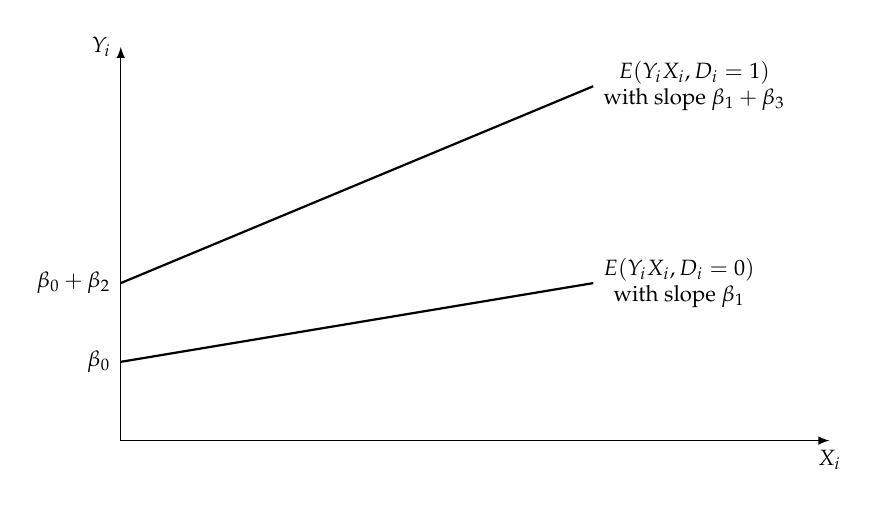
\begin{tikzpicture}[font=\footnotesize,>=latex]
    \draw[thick](0,1)node[left]{$\beta_0$}--(6,2)node[right,align=center]{$E(Y_i\given X_i,D_i=0)$\\with slope $\beta_1$};
    \draw[thick](0,2)node[left]{$\beta_0+\beta_2$}--(6,4.5)node[right,align=center]{$E(Y_i\given X_i,D_i=1)$\\with slope $\beta_1+\beta_3$};
    \draw[<->](0,5)node[left]{$Y_i$}--(0,0)--(9,0)node[below]{$X_i$};
  \end{tikzpicture}
  \end{center}
  
  \item Difference in slopes $\frac{\partial E(Y_i\given X_i,D_i)}{\partial X_i}$ between $E(Y_i\given X_i,D_i=1)$ and $E(Y_i\given X_i,D_i=0)$.
\end{enumerate}



7. Stock \& Watson 7.2
\begin{enumerate}
  \item The $t$-statistic is $8.31/0.23=36.1>1.96$, so the coefficient is statistically significant at the $5\%$ level.
  The $95\%$ confidence interval is $8.31\pm (1.96\times0.23)$.
  
  \item The $t$-statistic is $-3.85/0.23=-16.7>1.96$, so the coefficient is statistically significant at the $5\%$ level.
  The $95\%$ confidence interval is $-3.85\pm (1.96\times0.23)$.
\end{enumerate}



9.
$\beta_1$ measures the expected unit change in $Y_i$ given a
one-percent change in $X_i$.
\vskip15pt


10. Stock \& Watson 8.7
\begin{enumerate}
\item 
\begin{inparaenum}[(i)]
\item $ln(Earnings)$ for females are, on average, 0.44 lower for men than for women.\\
\item The error term has a standard deviation of 2.65 (measured in log-points).\\
\item Yes. But the regression does not control for many factors (size of firm, industry, profitability, experience and so forth).\\
\item No. In isolation, these results do not imply gender discrimination. Gender discrimination means that two workers, identical in every way but gender, are paid different wages. Thus, it is also important to control for characteristics of the workers that may affect their productivity (education, years of experience, etc.) If these characteristics are systematically different between men and women, then they may be responsible for the difference in mean wages. (If this were true, it would raise an interesting and important question of why women tend to have less education or less experience than men, but that is a question about something other than gender discrimination.) These are potentially important omitted variables in the regression that will lead to bias in the OLS coefficient estimator for Female.\\
Since these characteristics were not controlled for in the statistical analysis, it is premature to reach a conclusion about gender discrimination.
\end{inparaenum}
\item
\begin{inparaenum}[(i)]
\item If MarketValue increases by 1\%, earnings increase by 0.37\%.\\
\item Female is correlated with the two new included variables and at least one of the variables is important for explaining $ln(Earnings)$. Thus the regression in part (a) suffered from omitted variable bias.
\end{inparaenum}
\item Forgetting about the effect or Return, whose effects seems small and statistically insignificant, the omitted variable bias formula (see equation (6.1)) suggests that Female is negatively correlated with $ln(MarketValue)$.
\end{enumerate}


\section{Intrumental Variables}
1. Stock \& Watson 12.5
\begin{enumerate}
\item Instrument relevance. $Z_i$ does not enter the population regression for $X_i$.

\item $\hat X_i$ will be perfectly collinear with $W_i$. Alternatively, the first stage regression suffers from perfect multicollinearity.

\item $W_i$ is perfectly multicollinear with the constant term.

\item $Z_i$ violates instrument exogeneity, because it's correlated with the error term.
\end{enumerate}


2. Stock \& Watson 12.9
\begin{enumerate}
\item There are other factors that could affect both the choice to serve in the military and annual earnings. One example could be education, although this could be included in the regression as a control variable. Another variable is “ability” which is difficult to measure, and thus difficult to control for in the regression. 

\item The draft was determined by a national lottery so the choice of serving in the military was random. Because it was randomly selected, the lottery number is uncorrelated with individual characteristics that may affect earning and hence the instrument is exogenous. Because it affected the probability of serving in the military, the lottery number is relevant.
\end{enumerate}

3. Stock \& Watson 12.10
\begin{align*}
\hat{\beta}_{1}^{TSLS}&=\frac{s_{ZY}}{s_{ZX}}\\
&\xrightarrow{p}\frac{cov(Z_{i},Y_{i})}{cov(Z_{i},X_{i})}\\
&=\frac{cov(Z_{i},\beta_{0}+\beta_{1}X_{i}+\beta_{2}W_{i}+u_{i})}{cov(Z_{i},X_{i})}\\
&=\frac{\beta_{1}cov(Z_{i},X_{i})+\beta_{2}cov(Z_{i},W_{i})}{cov(Z_{i},X_{i})}
\end{align*}

\begin{enumerate}
\item If $cov(Z_{i},W_{i})=0$, $\hat{\beta}_{1}^{TSLS}\xrightarrow{p}\beta_{1},$
the IV estimator is consistent.
\item If $cov(Z_{i},W_{i})\neq0$, $\hat{\beta}_{1}^{TSLS}\xrightarrow{p}\frac{\beta_{1}cov(Z_{i},X_{i})+\beta_{2}cov(Z_{i},W_{i})}{cov(Z_{i},X_{i})},$
the IV estimator is not consistent.
\end{enumerate}

\end{document}